%!TEX root = ../dissertation.tex

\hypertarget{(chap:inquadramento)}{}
\chapter{Test}
Una attività di fondamentale importanza è stata quella di testare i modelli e archiviare i dati.
\section{Istanze}
Una \glo{istanza} è un insieme formato dai pacchi da disporre nel contenitore e il contenitore stesso.\\
Un gruppo di istanze è un insieme di istanze diverse tra loro accomunite tra loro dalle dimensioni simili o dal numero di oggetti.\\
Inizialmente ogni qual volta testavamo un modello dopo aver apportato una modifica, eseguivamo un centinaio di test con un gruppo di istanze completamente randomico, l'obiettivo in questo caso era quello di individuare imperfezioni o testare la tenuta dei vincoli.
Successivamente si passava all'esecuzione di 100 test per ciascuna delle istanze riportate di seguito.
\begin{center}
	\begin{tabular}{lrrrr}
		\toprule
		{} & width\_a & width\_b & depth\_a & depth\_b \\
		\midrule
		0  & 0.5      & 2.45     & 0.5      & 2.45     \\
		1  & 0.5      & 1.50     & 0.5      & 4.00     \\
		2  & 1.5      & 2.45     & 0.5      & 4.00     \\
		3  & 0.5      & 1.50     & 3.0      & 4.00     \\
		4  & 1.5      & 2.45     & 3.0      & 4.00     \\
		5  & 0.1      & 1.00     & 0.1      & 1.00     \\
		6  & 0.1      & 1.00     & 3.0      & 4.00     \\
		7  & 2.0      & 2.45     & 3.0      & 4.00     \\
		8  & 2.0      & 2.45     & 2.0      & 2.45     \\
		9  & 0.1      & 1.00     & 0.1      & 4.00     \\
		\bottomrule
	\end{tabular}
	\captionof{table}{Le dimensioni dei gruppi di istanze eseguite}
\end{center}
La tabella riporta gli intervalli entro cui si è deciso randomicamente le dimensioni dei pacchi, ogni gruppo di istanze aveva dimensioni particolari entro cui dovevano trovarsi i pacchi:
\begin{itemize}
	\item \textbf{Larghezza}: [width\_a, width\_b]
	\item \textbf{Profondità}: [depth\_a, depth\_b]
\end{itemize}
\section{Numero di oggetti}
Fin dal modello 2D abbiamo capito che il numero di pacchi per ogni istanza sarebbe stato in numero limitato in quanto dopo 7 pacchi i tempi di esecuzione esplodevano, abbiamo quindi deciso di scegliere in modo randomico in un intervallo [3,10] il numero di pacchi da assegnare a ciascuna istanza, imponendo un \glo{time limit} di 300 secondi, questo portava ad ottenere soluzioni ottime e soluzioni \glo{best bound}, l'analisi dei risultati sarà divisa in queste due categorie infatti.

\begin{figure}[!ht]
	\begin{center} 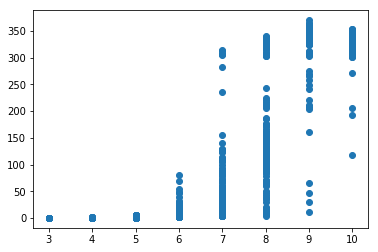
\includegraphics[scale=0.8]{figures/time_nitems}
		\caption[Bin packing figures]{Due contenitori completamente pieni}  
		\label{fig:times}
	\end{center}
\end{figure}

Nel grafico sopra riportato~\eqref{fig:times} viene riportato come ordinata il numero di oggetti e sull'ascissa il tempo espresso in secondi, come si può vedere man mano che gli oggetti aumentano il tempo aumenta notevolmente passando da pochi secondi a minuti, risultano molto interessanti quelle istanze che nonostante abbiano molti oggetti richiedano meno tempo per essere eseguiti, forse questo dovuto alle particolari dimensioni degli oggetti.